\documentclass[letterpaper]{article}

\usepackage[top=1in, bottom=1in, left=1in, right=1in]{geometry}
\usepackage{float}
\usepackage{graphicx}
\usepackage{caption}
\usepackage{subcaption}
\usepackage{amsmath}
\usepackage{fancyhdr}
\usepackage{hyperref}

\setlength{\headheight}{15.2pt}

\pagestyle{fancy}
\lhead{Water Runner Simulation}
\lfoot{Nitish Thatte}
\cfoot{\thepage}
\rfoot{\today}

\title{Water Runner Simulation}
\author{Nitish Thatte}

\begin{document}
\maketitle

\section{Foot Forces/Moments}
\subsection{Water Running}
The water runner robot can locomote on water by plunging its footpads into the liquid at high velocities generating lift and thrust. The drag on the foot is approximated by the drag on a disk entering water vertically given by:

\begin{equation}
	D(t) = C_D^* [0.5 S \rho u^2 + S \rho g h(t)]
\end{equation}

\noindent Where $C_D^* \approx 0.703$ is the coefficient of drag, $\rho$ is the density of water, $u$ is the foot speed, $S = \pi r_{eff}^2$, and $h(t)$ is the depth of the foot under the water \cite{Glasheen1996a}. The integral of this drag pressure over the submerged area of the foot gives the total force $(F_w)$ and moment $(M_w)$ on the foot:

\begin{align}
F_w &= C_D^* \int_{-R}^{-R+2pR} \sqrt{R^2 - s^2} (2gh(s) + a(s)|a(s)|) ds \label{eq:footF}\\
M_w &= C_D^* \rho \int_{-R}^{-R + 2pR} \sqrt{R^2 - s^2} (2gh(s) + a(s)|a(s)|)(-s) ds \label{eq:footM} \\
a(s) &= \vec{v}(s) \cdot \vec{n} \\
h(s) &= (y_\mathrm{water} - y_\mathrm{BF} ) \left( 1 - \frac{s + R}{2 p R} \right)
\end{align}

\noindent Where $s$ is a point along the length of the foot, $\vec{v}(s)$ is the velocity of the point $s$, $\vec{n}$ is the footpad's normal vector, $h(s)$ is the depth of point $s$, $p$ is the percent of the footpad that is submerged, and $F_w$ and $M_w$ are the total force and moment on the foot respectively \cite{Floyd2008}.

In order to reduce drag while withdrawing the foot from the water, the footpads feature a breakaway mechanism that folds when $a(s) < 0$, i.e. the component of the foot velocity normal to the footpad points down from above the foot. The reduction in area in this state is approximated by a reduction in the footpad radius to $1/4^\textrm{th}$ its original value \cite{Floyd2009}. The folded foot area also causes an additional drag force. This added force is modeled by the drag created by a footpad, with equal radius and orthogonal to the original footpad.

\subsection{Ground Running with Compliant Feet}
While rigid feet are desirable during water running as they ensure the robot presents the maximum area footpad area to the water and thus and generates the maximum drag possible during the downwards stroke phase, compliant feet are better suited for hard ground running. This is because spring-like feet can store kinetic energy as potential energy during ground impact and  then release it again during liftoff. Compliant rubber feet have been developed for the water running robot to assess its running performance on hard ground.

To simplify the bending dynamics of the compliant rubber foot, it is approximated via a pseudo-rigid body model as two rigid links with an appropriately placed torsional spring.  Using this model, the dynamics of the compliant foot can be modeled with the following equation:

\begin{equation}
	I_{eff} \ddot{\theta} = -b\dot{\theta} - k\theta + M
\end{equation} 

Where $\theta$ is the compression angle of the torsional spring, $b$ is the damping constant, $k$ is the stiffness constant, $M$ is the bending moment at the location of the torsional spring, and $I_{eff}$ is the effective inertia of the pseudo-rigid foot. This term, as well as $b$ and $k$ are found experimentally \cite{Park2009}. In order to find $M$ we need to know the forces where the foot contacts the ground. These are given by the following ground contact model:

\begin{equation}
F_y = \left\{ \begin{array}{ll} 0.25 \times 10^9 |y_p|^3 (1 - \dot{y}_p) & \quad \textrm{if $y_p > 0$} \\ 0 & \quad \textrm{if $y_p \le 0$} \end{array} \right.
\end{equation}

\noindent Forces in the $x$-direction can be calculated using via a standard dry friction model:

\begin{equation}
F_x = \left\{ \begin{array}{ll} m_r a_x & \quad \textrm{if $m_r a_x < \mu_s F_y$} \\
			                   \mu_k F_y &\quad \textrm{if $m_r a_x \ge \mu_s F_y$}
			  \end{array} \right.
\end{equation}


\section{Leg Four Bar Angle Calculations}

The leg of the water runner robot is a crank-rocker four-bar mechanism and can be seen in figure \ref{fig:4bar}.
\begin{figure}[htb]
	\centering
	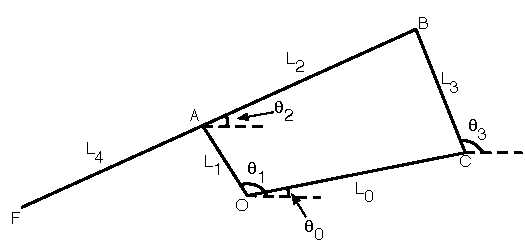
\includegraphics[width = 0.5\textwidth]{4bar.pdf}
	\caption{Labeled 4-bar leg mechanism.}
	\label{fig:4bar}
\end{figure}

\subsection{Angular Position}
Given $\theta_1$, angles $\theta_2$ and $\theta_3$ can be obtained as follows. First, we write the relationship between points $A$ and $B$ on the four bar linkage

\begin{equation}
	(B - A)^2 - L_2^2 = 0
	\label{eq:BArel}
\end{equation}

\begin{align}
	A &= \begin{bmatrix} L_1 \cos \theta_1 \\ L_1 \sin \theta_1 \end{bmatrix}   \label{eq:Aloc}\\
	B &= \begin{bmatrix} L_0 \cos \theta_0 \\ L_0 \sin \theta_0 \end{bmatrix} 
			+ \begin{bmatrix} L_3 \cos \theta_3 \\ L_3 \sin \theta_3 \end{bmatrix} \label{eq:Bloc}
\end{align}

\noindent Plugging equations \ref{eq:Aloc} and \ref{eq:Bloc} into \ref{eq:BArel} yields
\begin{align}
	0 &= (L_0 \cos \theta_0 + L_3 \cos \theta_3 - L_1 \cos \theta_1)^2 + (L_0 \sin \theta + L_3 \sin \theta_3 - L_1 \sin \theta_1)^2 - L_2^2 \notag \\
	  &= L_0^2 \cos^2 \theta_0 + 2 L_0 L_3 \cos \theta_0 \cos \theta_3 - 2 L_0 L_1 \cos \theta_0 \cos \theta_1 + L_3^2 \cos^2 \theta_3 - 2 L_1 L_3 \cos \theta_1 \cos \theta_3 + L_1^2 \cos^2 \theta_1 \notag \\
	  & \quad  + L_0^2 \sin^2 \theta_0 + 2 L_0 L_3 \sin \theta_0\ \sin \theta_3 -2 L_0 L_1 \sin \theta_0 \sin \theta_1 + L_3^2 \sin^2 \theta_3 - 2 L_1 L_3 \sin \theta_3 \sin \theta_1 + L_1^2 \sin^2 \theta_1 - L_2^2 \notag \\
	  &= L_0^2 + L_3^2 + L_1^2 - L_2^2 - 2 L_0 L_1 \cos \theta_0 \cos \theta_1 \notag \\
	  &  \quad + 2 L_0 L_3 \cos \theta_0 \cos \theta_3 - 2 L_1 L_3 \cos \theta_3 \cos \theta_1 \notag \\
	  &  \quad + 2 L_0 L_3 \sin \theta_0 \sin \theta_3 - 2 L_1 L_3 \sin \theta_3 \sin \theta_1
\end{align}

\noindent Grouping the terms that do not depend on $\theta_3$,

\begin{align}
	\alpha &= 2 L_0 L_3 \cos \theta_0 - 2 L_1 L_3 \cos \theta_1 \\
	\beta &=  2 L_0 L_3 \sin \theta_0 - 2 L_1 L_3 \sin \theta_1 \\
	\gamma &= L_0^2 + L_3^2 + L_1^2 - L_2^2 - 2 L_0 L_1 \cos \theta_0 \cos \theta_1 - 2 L_0 L_1 \cos \theta_0 \cos \theta_1
\end{align}

\noindent If we define $\delta = \tan^{-1} \left( \frac{\beta}{\alpha} \right)$ then it follows that

\begin{equation}
	\cos \delta \cos \theta_3 + \sin \delta \sin \theta_3 + \frac{\gamma}{\sqrt{\alpha^2 + \beta^2}} = 0
\end{equation}

\noindent Therefore, 

\begin{align}
	\theta_3 &= \delta \pm \cos^{-1} \left( \frac{- \gamma}{\sqrt{\alpha^2 + \beta^2}} \right) \\
	\theta_2 &= \tan^{-1} \left( \frac{ L_0 \sin \theta_0 + L_3 \sin \theta_3 - L_1 \sin \theta_1}{L_0 \cos \theta_0 + L_3 \cos \theta_3 - L_1 \cos \theta_1} \right)
\end{align}

\subsection{Angular Speed}

Loop closure requires that

\begin{align}
	A + (B - A) &= C + (C - B) \notag \\
	\frac{d}{dt} A - \frac{d}{dt} (B - A) &= \frac{d}{dt} C + \frac{d}{dt} (B - C) \label{eq:dloop}\\
\end{align}

\noindent Rearranging terms yields a system of linear equations that allows us to solve for $\dot{\theta}_3$ and $\dot{\theta}_2$ given $\dot{\theta}_1$, and $\dot{\theta}_0$,

\begin{equation}
	\begin{bmatrix} -L_3 \sin \theta_3 && L_2 \sin \theta_2 \\ L_3 \cos \theta_3 && - L_2 \cos \theta_2 \end{bmatrix} \begin{bmatrix} \dot{\theta}_3 \\ \dot{\theta}_2 \end{bmatrix} = \begin{bmatrix} -L_0 \sin \theta_0 \\ L_0 \cos \theta_0 \end{bmatrix} \dot{\theta}_0 + \begin{bmatrix} -L_1 \sin \theta_1 \\ L_1 \cos \theta_1 \end{bmatrix} \dot{\theta}_1
\end{equation}

\subsection{Angular Acceleration}

Differentiating the velocity loop closure equation (\ref{eq:dloop}) yields:

\begin{equation}
	\frac{d^2}{dt^2} A + \frac{d^2}{dt^2} (B -A) = \frac{d^2}{dt^2} C + \frac{d^2}{dt^2} (B - C) \\
\end{equation}

\noindent Again, rearranging terms yields a system of linear equations that allows us to solve for $\ddot{\theta}_3$ and $\ddot{\theta}_2$ given $\ddot{\theta}_0$, $\ddot{\theta}_1$, $\dot{\theta}_0$, $\dot{\theta}_1$, $\dot{\theta}_2$, $\dot{\theta}_3$, $\theta_0$, $\theta_1$, $\theta_2$, and $\theta_3$,

\begin{align}
	\begin{bmatrix} -L_3 \sin \theta_3 && L_2 \sin \theta_2 \\ L_3 \cos \theta_3 && -L_2 \cos \theta_2 \end{bmatrix} \begin{bmatrix} \ddot{\theta}_3 \\ \ddot{\theta}_2 \end{bmatrix} &= \begin{bmatrix} L_0 \sin \theta_0 \\ - L_0 \cos \theta_0 \end{bmatrix} \ddot{\theta}_0 + \begin{bmatrix} -L_1 \sin \theta_1 \\ L_1 \cos \theta_1 \end{bmatrix} \ddot{\theta}_1 \notag \\
		& \quad + \begin{bmatrix} L_0 \cos \theta_0 \\ L_0 \sin \theta_0 \end{bmatrix} \dot{\theta}_0^2- \begin{bmatrix} L_1 \cos \theta_1 \\ L_1 \sin \theta_1 \end{bmatrix} \dot{\theta}_1^2 - \begin{bmatrix} L_2 \cos \theta_2 \\ L_2 \sin \theta_2 \end{bmatrix} \dot{\theta}_2^2 + \begin{bmatrix} L_3 \cos \theta_3 \\ L_3 \sin \theta_3 \end{bmatrix} \dot{\theta}_3^2
\end{align}

\section{Force/Torque calculations}

\begin{figure}[htb]
	\centering
	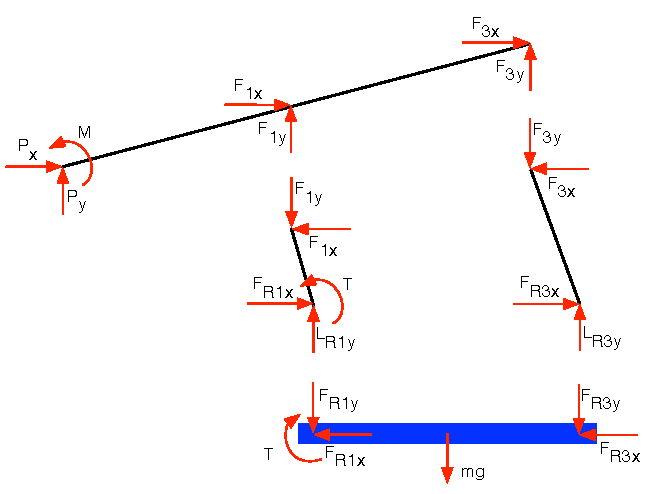
\includegraphics[width = 0.5\textwidth]{FB.pdf}
	\caption{Free body diagrams of forces and moments on each link and the robot (in blue).}
	\label{fig:FB}
\end{figure}

To calculate the forces and torques on the leg joints, we start by assuming the links in the leg's four bar mechanism are massless. Therefore, the forces and moments on each link must sum to zero. These force and moment summations result in a system of linear equations, shown below, that can be solved to obtain the forces on each joint as well as the torque on the motor shaft.

\begin{equation}
\begin{bmatrix}
0 & 0 & 0 & 0 & 1 & 0 & 1 & 0 &0 \\ 
0 & 0 & 0 & 0 & 0 & 1 & 0 & 1 &0 \\
0 & 0 & 0 & 0 &  -L_4 \sin \theta_2 &  L_4 \cos \theta_2& -(L_2 + L_4) \sin \theta_2 & (L_2 + L_4) \cos \theta_2 & 0 \\
1 & 0 & 0 & 0 & -1 & 0 & 0 & 0 & 0 \\
0 & 1 & 0 & 0 & 0 & -1 & 0 & 0 & 0 \\
0 & 0 & 0 & 0 & L_1 \sin \theta_1 & -L_1 \cos \theta_1 & 0 & 0 & 1\\
0 & 0 & 1 & 0 & 0 & 0 & -1 & 0 & 0 \\
0 & 0 & 0 & 1 & 0 & 0 & 0 & -1 & 0 \\
0 & 0 & 0 & 0 & 0 & 0 & L_3 \sin \theta_3 & -L_3 \cos \theta_3 & 0
\end{bmatrix}
\begin{bmatrix} F_{R1x} \\ F_{R1y} \\ F_{R3x} \\ F_{R3y} \\ F_{1x} \\ F_{1y} \\ F_{3x} \\ F_{3y} \\ T \end{bmatrix}
=
\begin{bmatrix} -P_x \\ - P_y \\ -M \\ 0 \\ 0 \\ 0 \\ 0 \\ 0 \\ 0 \end{bmatrix}
\end{equation}

\subsection{Robot Forces/Torques}
Once the forces on the legs are calculated, the relevant forces are transmitted to the robot through the following equations

\begin{align}
	\sum F_x &= m \ddot{x} = -F_{R1x} - F_{R3x}  \\
	\sum F_y &= m \ddot{y} = -F_{R1y} - F_{R3y} - mg \\
	\sum M_{COM} &= I \ddot{\theta}_0 = -F_{R1y} L_{COM} \cos \theta_0 + F_{R1x} L_{COM} \theta_0 \notag \\
		& \phantom{I \ddot{\theta}_0 =} \qquad - F_{R3y} (L_{COM} - L_0) \cos \theta_0 + F_{R3x} (L_{COM} - L_0) \sin \theta_0 - T
\end{align}



\noindent These equations are then integrated to obtain the motion of the robot.

\section{Numerical Methods}

A design requirement for the simulator is that it allow for easy swapping of components simply by replacing objects in the code with different ones. For example, switching from the circular foot used for water running to the compliant rubber foot used for ground running simply requires loading the respective class for each type of foot. A side effect of this design is that it makes tracking the state of individual components at a high level in the program difficult, as each component keeps track of its own state and only passes relevant forces and constraints to its connected components. As a result, the simulation, at the robot-level, can only move forward in time.

This became a problem as it prevented the use of some numerical methods that require multiple steps and backtracking. For example, in the Runge-Kutta method the current derivative is used to step forward in time and obtain future derivatives. Then, these derivatives are averaged to produce the final derivative used for that timestep. However, using this method on the robot is not possible as once the state of the robot is advanced it cannot be reversed.  Instead, the Adam's-Bashforth method is used to integrate the calculated acceleration of the robot because it does not use future timesteps to calculate the current derivative. Rather, it estimates the future derivatives by interpolating from past and current information.

Another numerical issue that arose was that the interaction between the relatively compliant foot and the hard ground resulted in a stiff system that required extremely small timesteps to solve. Ideally, an implicit method would be used to integrate such a system, but due to the issues outlined above, these methods were infeasible. However, it was possible to use a Runge-Kutta method, which provides an order of magnitude improvement over Adam's Bashforth, to integrate the foot as it is the last component connected to the robot and does not have any child components. Small time steps were also required for the foot even when it was not in contact with the ground because the vibration dynamics of the foot occur on timescales much smaller than those at which the robot dynamics occur. Therefore, Runge-Kutta is used to independently integrate the foot at a very fine timestep, while the robot is integrated at a much coarser timestep. 

Additionally, to prevent the tip of the foot from penetrating too far into the ground surface during initial contact, an adaptive timestep was used to reduce the timestep of the robot's Adam's-Bashforth method to that of the foot's Runge-Kutta method while the tip of the foot was less than some height above the ground. This adaptive-multirate solution yielded stable results and an acceptable time for most situations. However, very fast collisions with the ground can still cause numerical issues even with these techniques.

\section{Conclusion}

This simulation should serve as a useful testbed for future development of this robotic platform. Additional features that can be added are an electro-mechanical model for the DC motors that drive the legs. This would provide additional dampening to the system and limit the amount of torque the motors can apply to the legs. Once this is feature is added, various gait control strategies could be tested and evaluated.

\bibliography{library.bib}{}
\bibliographystyle{plain}


\end{document}
